\chapter{Method}\label{cha:method}

This chapter will describe the pipeline of the algorithm developed during this master thesis. The different parts of the algorithm are viewed with a more implementation focused view.

\section{Overview}

An overview of the algorithm is presented in figure \ref{fig:detection_flow}. The algorithm start of with pre-processing an input image. This step makes sure that the image is normalized and that all necessary sub-parts are generated. Then a facial mask is generated in the segmentation step. Now the algorithm have everything in order to detect the skin mark candidates. All the candidates are then post-processed to eliminate false detections. Finally, the remaining skin marks are classified as a permanent or non-permanent skin mark.    

\FloatBarrier
 \begin{figure}[h]
 	\centering
 	
\includegraphics[width=\textwidth,height=\textheight,keepaspectratio]{flow_report}
 	\caption{Overview of the algorithm \label{fig:detection_flow}}
 \end{figure}
\FloatBarrier

\section{Data and annotation}

To evaluate the algorithm, a set of 106 images of faces en face were acquired from SCface database \cite{SCface} and FRGC database \cite{FRGC}. These images where collected at University of Zagreb and University of Notre Dame respectively. The purpose of the databases is to provide data to develop and improve face recognition algorithms. The images where taken in under controlled conditions indoor in a studio setting indoor with a high-quality photo camera. Figure \ref{fig:orig_img} shows an example of the images from the databases.

\FloatBarrier
\begin{figure}[h]
	\centering
	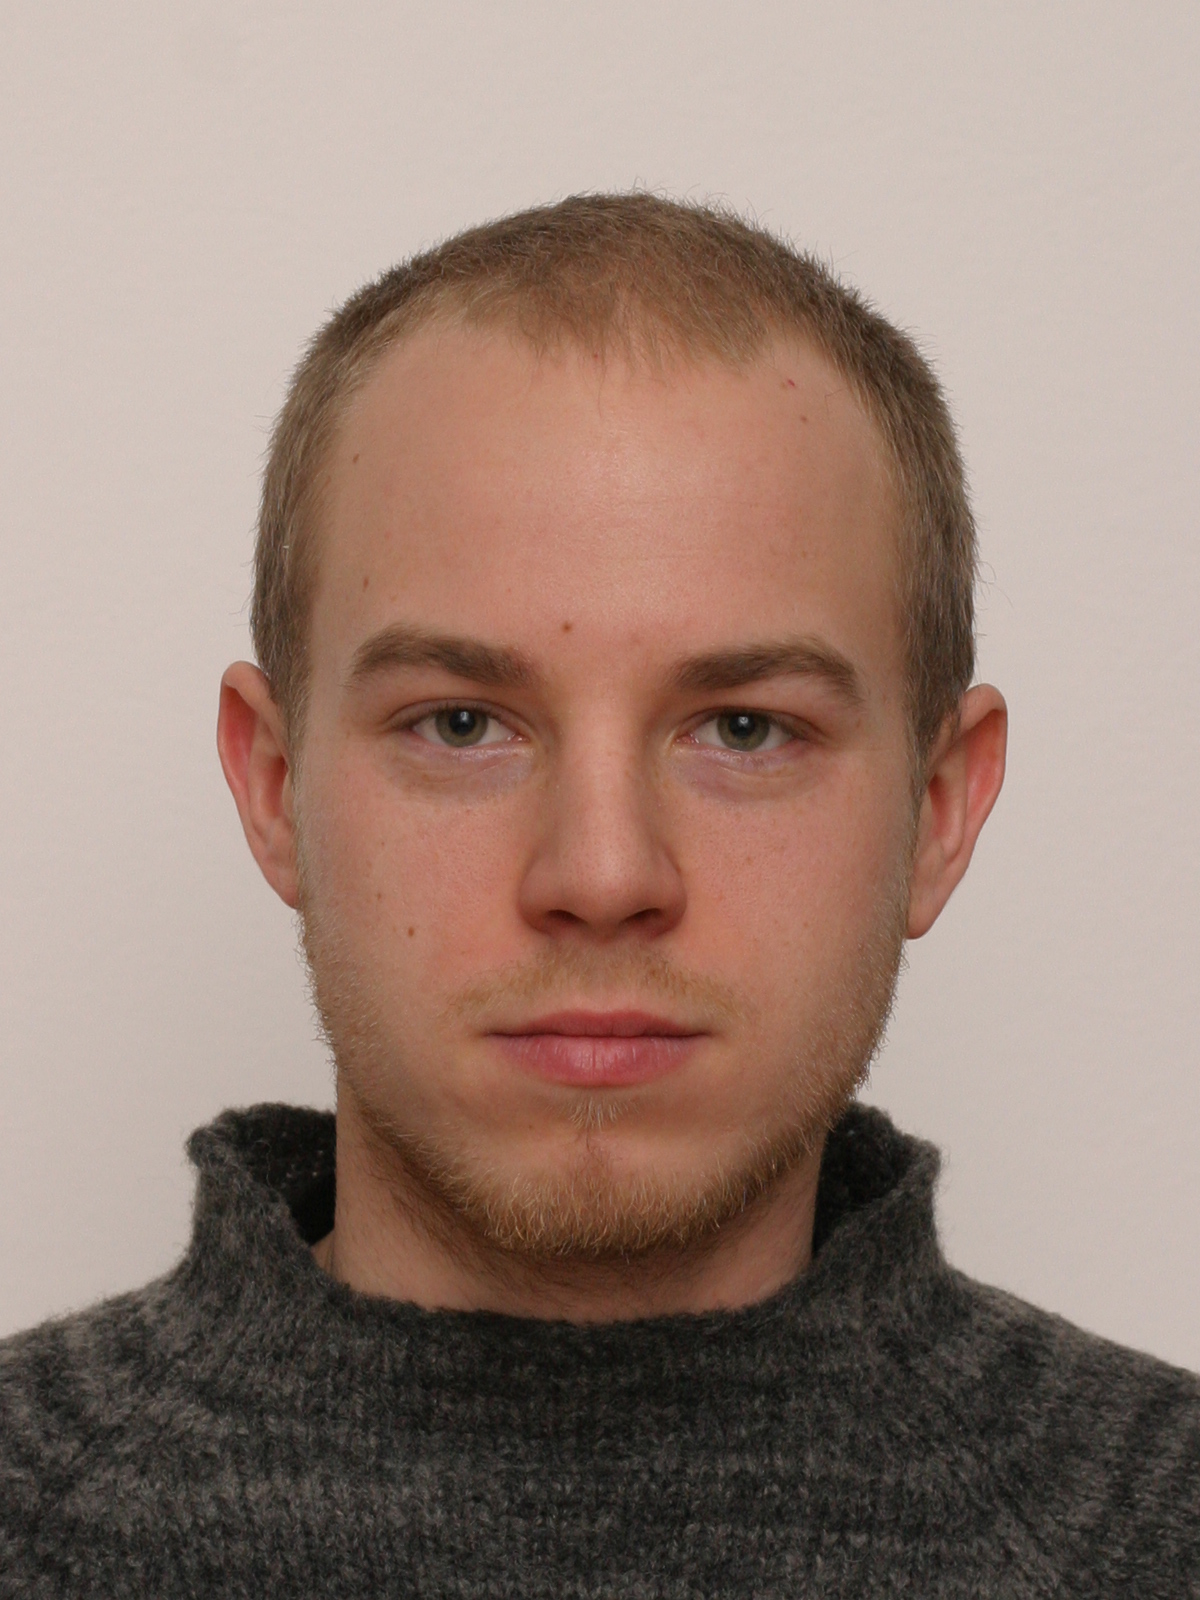
\includegraphics[width=\textwidth/2,height=\textheight/2,keepaspectratio]{001_orig}
	\caption{One example of the images used to evaluate the algorithm \label{fig:orig_img}}
\end{figure}
\FloatBarrier

Each image was examined the supervisors at NFC who labeled facial skin mark of interest. Each mark was given either the label permanent or non-permanent according to NFC definitions. This resulted in 506 marks where 353 were labeled as permanent and 153 non-permanent. 

\section{Pre-processing}

When the algorithm is given a RGB image, denoted $I$, it first detects the location of the face with the help of the face detector in OpenCV. It surrounds the face with a bounding box. With the bounding box, the facial landmarks can be detected by using the algorithm from Dlib. This landmark algorithm was chosen since it converges faster than other state of the art methods \cite{dlib_landmark}. 

\FloatBarrier
\begin{figure}[!h]
	\centering
	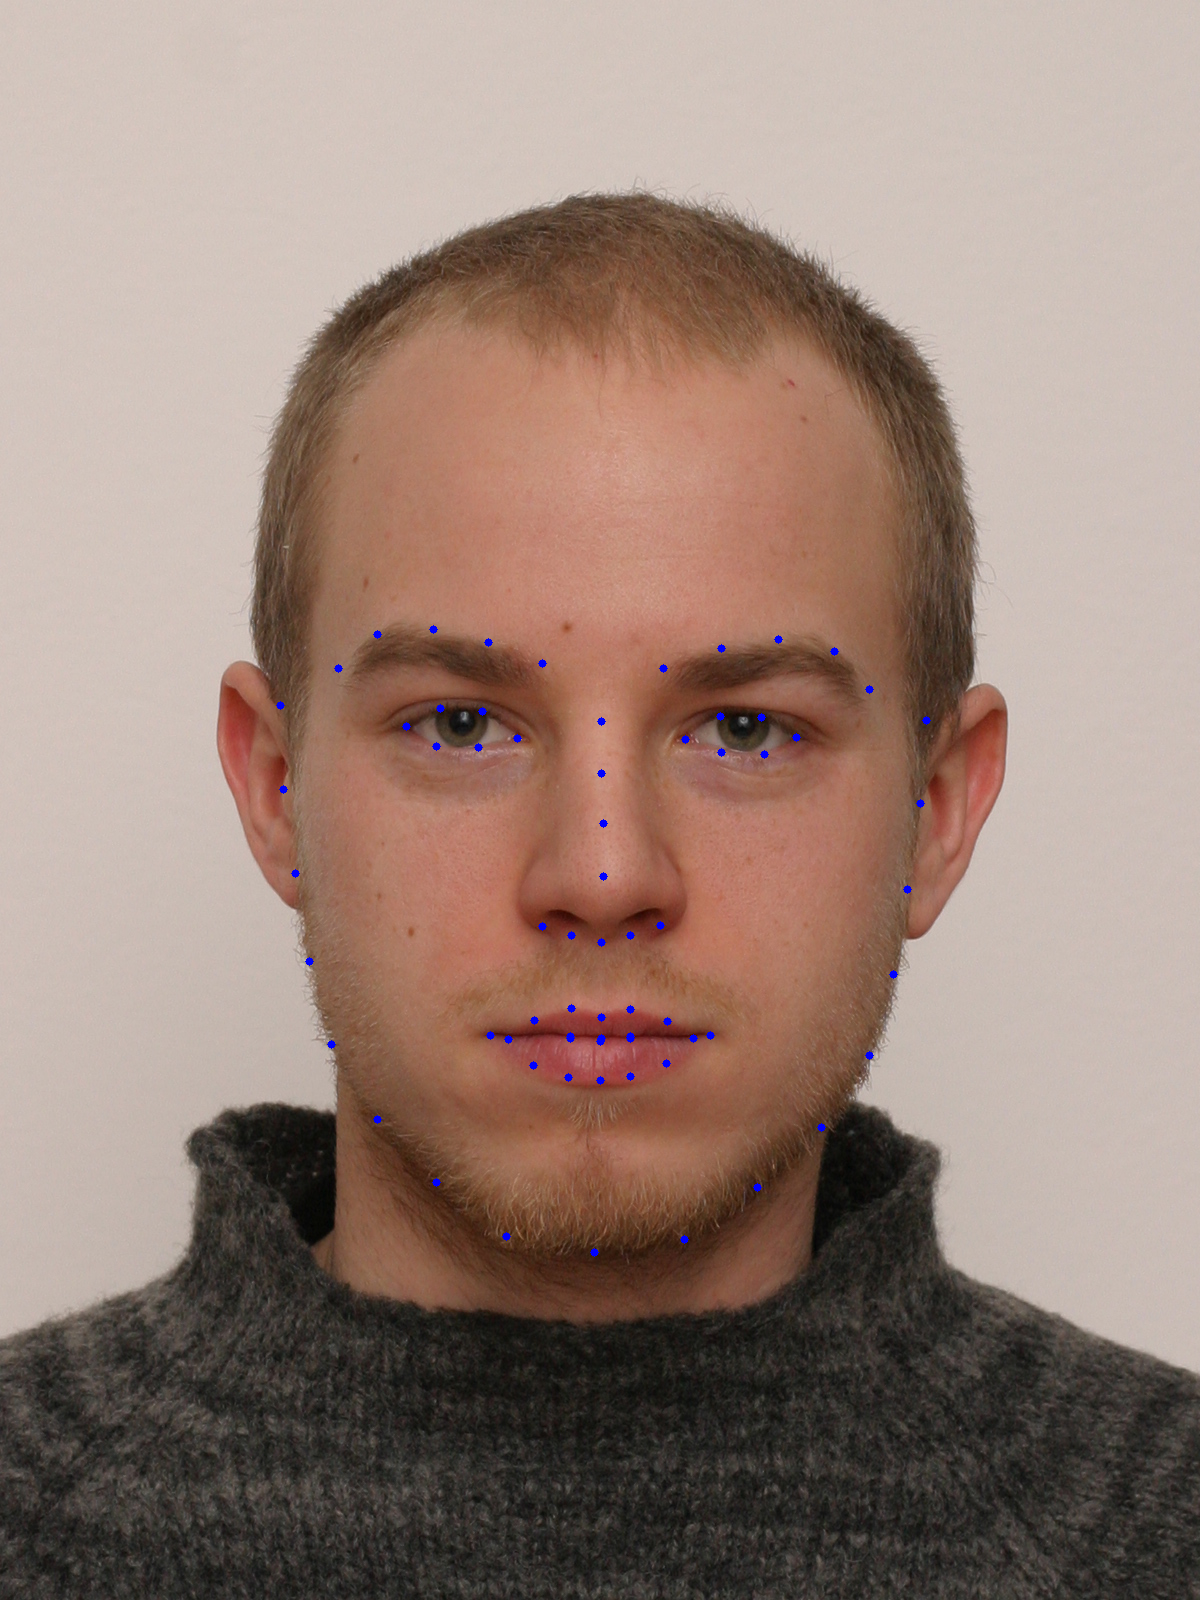
\includegraphics[width=\textwidth/2,height=\textheight/2,keepaspectratio]{landmarks}
	\caption{Image with the 64 landmarks shown as blue dots \label{fig:landmarks}}
\end{figure}
\FloatBarrier

With the landmarks, it is possible to begin the normalization process, see \cref{sec:normalization}. First, the image is photometric normalized using LRSR algorithm. This tone mapping operator is fast and had a good implementation available in C++. It performs on pair with the best tone mapping operator of today \cite{badger}. Photometric normalization is vital since the visibility of facial marks can be affected by varying illumination of the image.  

Second, the image is rescaled such that the interpupillary distance is 500 pixels. This resizes the images to approximately 2100x2800 and the interpolation method used is cubic interpolation. The landmarks are also used to rotate the image so that the eyes are level. The rotation and resizing of the image is called geometric normalization and is necessary remove the effect of the distance and tilt of the camera. In \cref{fig:rotated_img} one can see the result from the image normalization. 

\FloatBarrier
\begin{figure}[!h]
	\centering
	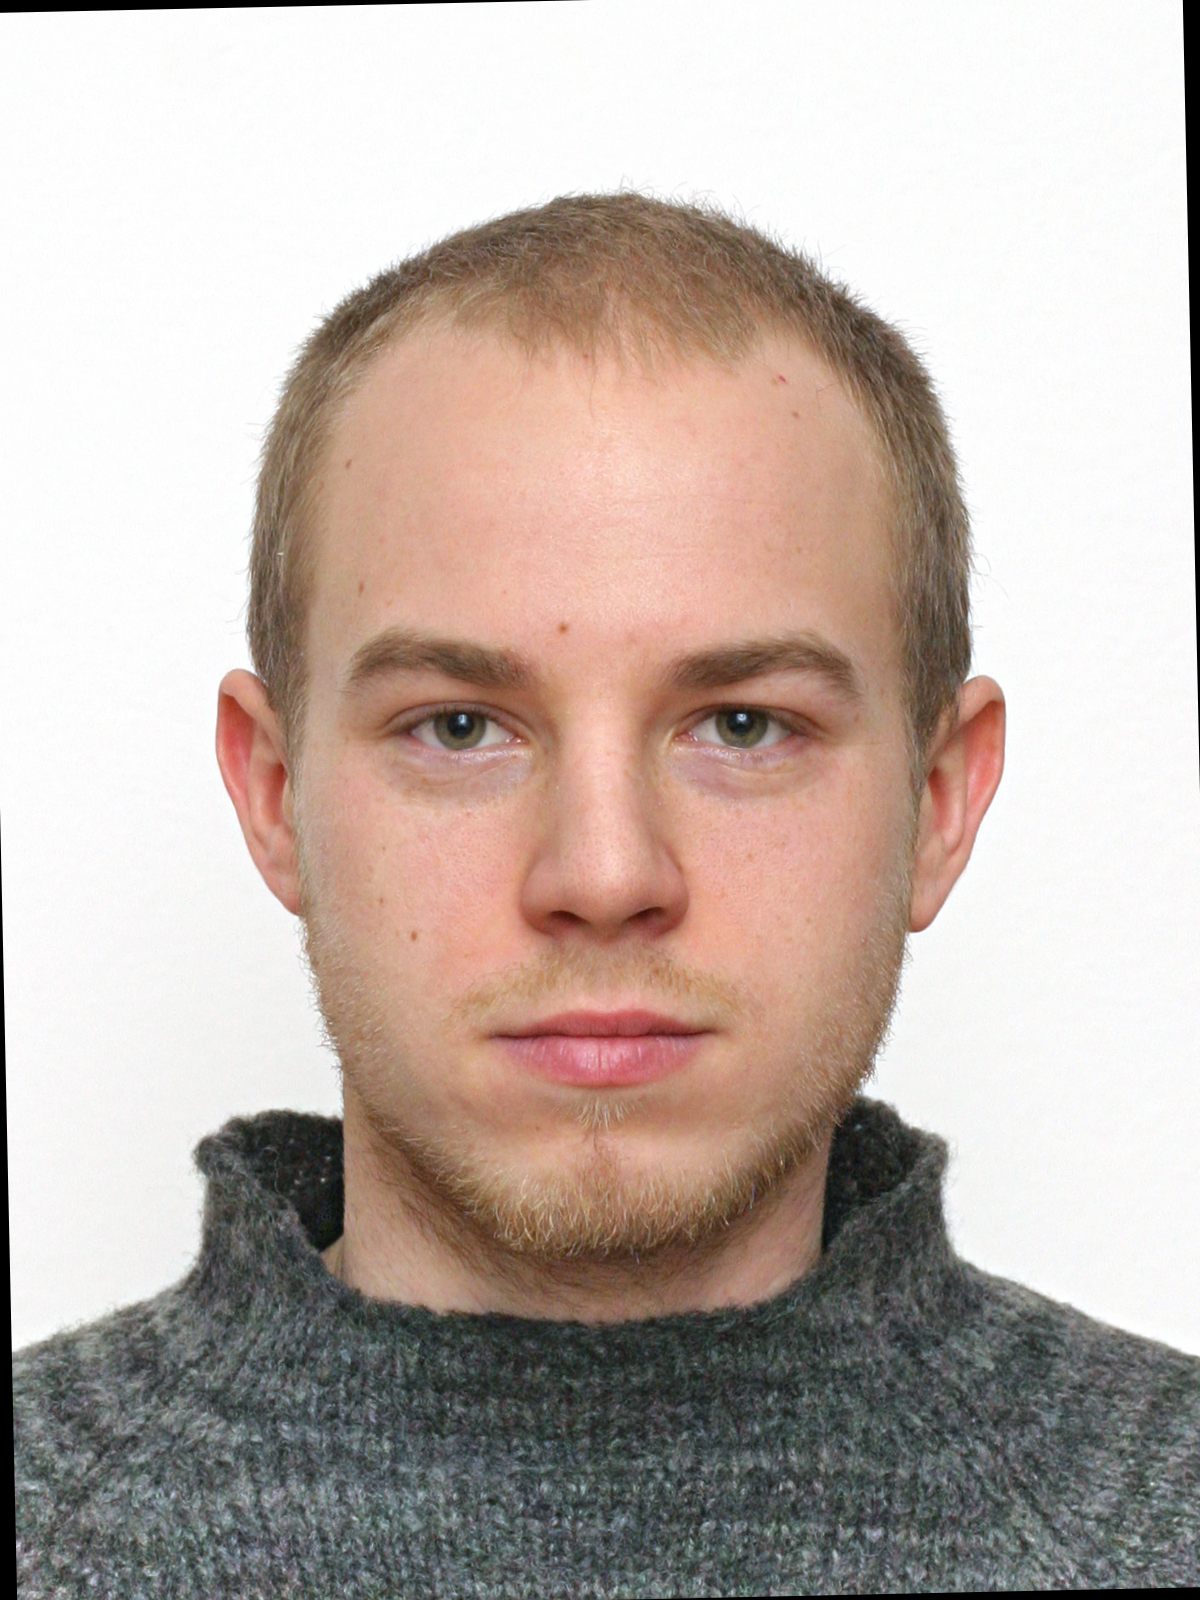
\includegraphics[width=\textwidth/2,height=\textheight/2,keepaspectratio]{001_rotated}
	\caption{Image after photometric and geometric normalization \label{fig:rotated_img}}
\end{figure}
\FloatBarrier

The last part of the pre-processing step is to segment out areas, see \cref{sec:segmentation}, which can cause false detections such as facial hair, nostrils, pupils etc. This is done by generating a binary mask. To segment out areas with skin, the implementation of GrabCut in OpenCV was used since it has proven to perform as well or better than many other user interactive foreground extraction methods \cite{grabcut}. From the skin mask, the eyes, nostrils, mouth and throat are cut out using elliptical shapes around the landmarks marking these regions. To expand these holes, a morphological erosion algorithm was performed on the image with a 3x3-kernel containing ones. The resulting mask can be observed in \cref{fig:mask_img}. 

\FloatBarrier
\begin{figure}[!h]
	\centering
	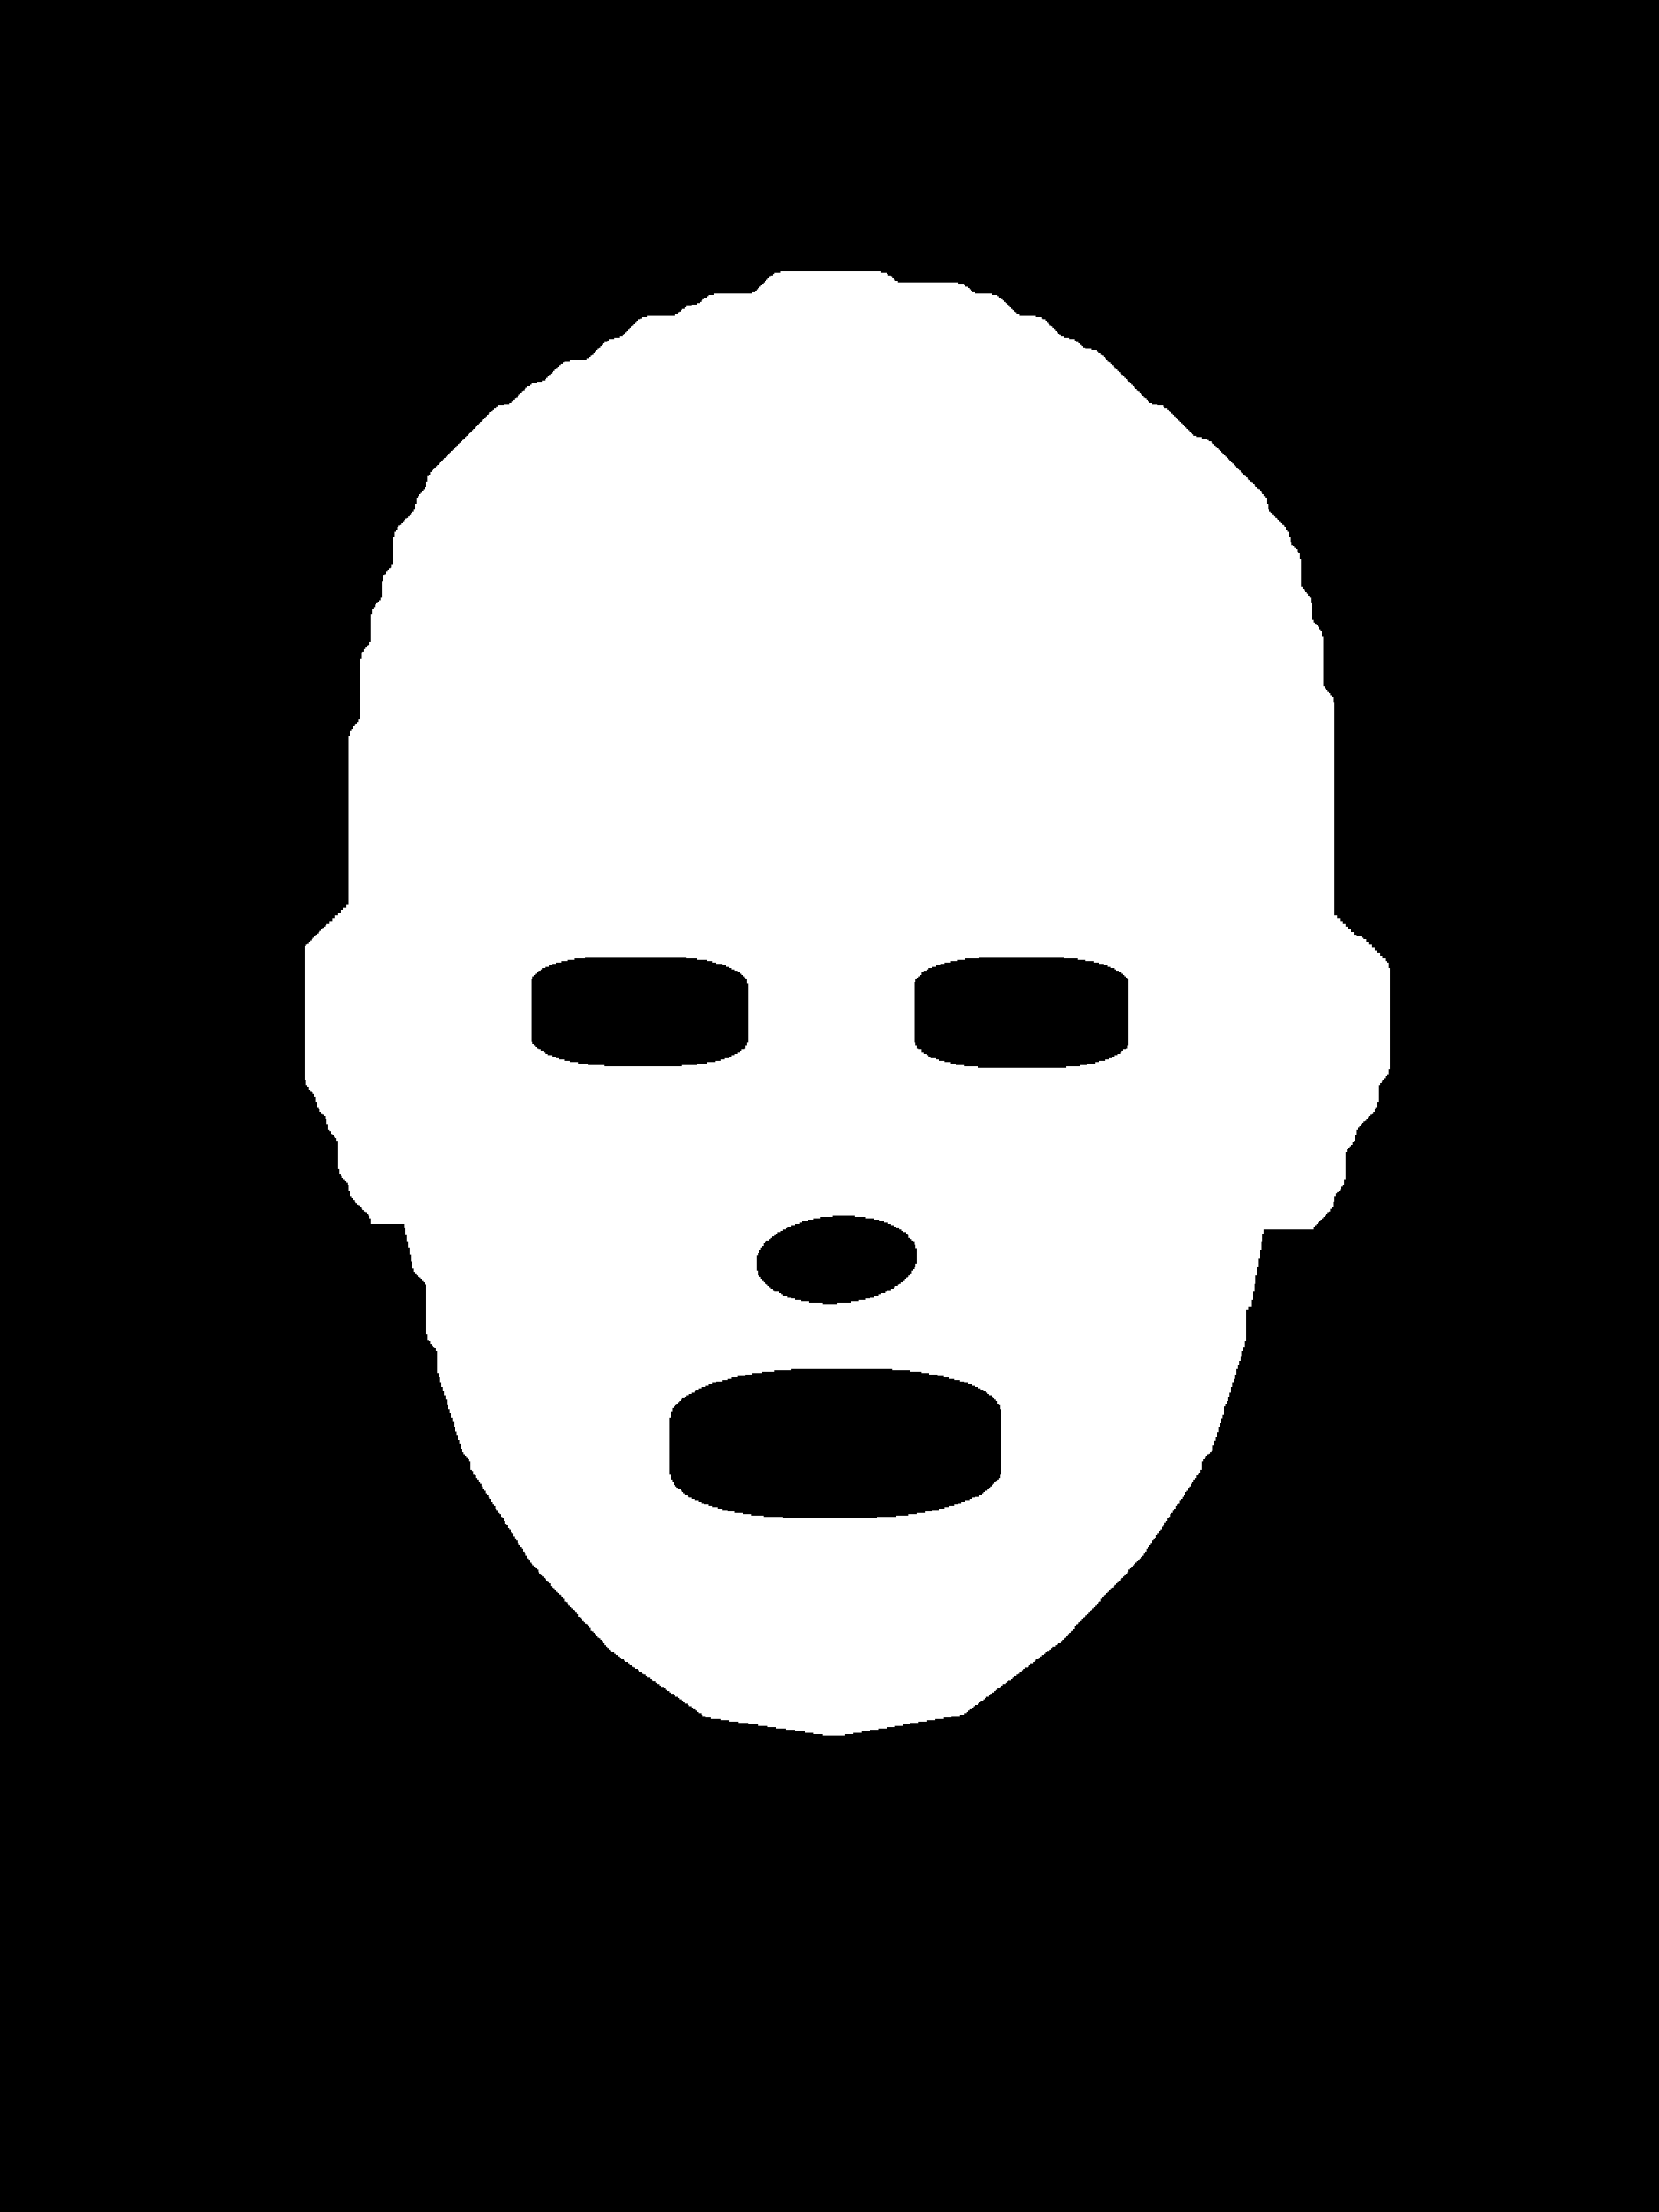
\includegraphics[width=\textwidth/2,height=\textheight/2,keepaspectratio]{001_mask}
	\caption{Image of the facial mask \label{fig:mask_img}}
\end{figure}
\FloatBarrier        

\section{Candidate detection}

The pre-processed image, denoted $I_{pre}$, can now be used to search for facial skin mark candidates. This is done with the help of FRS algorithm, see \cref{sec:FRS}. It highlights circular shapes which can be more easily detected. The algorithm makes calculations with different radii, $N$, and the ones used are $N = \{1, 3, 5, 7, 9, 11, 13, 15 \}$. These radii were used since 75\% of facial marks had an area smaller than 600 pixels, see \cref{fig:result_box_size}. The Gaussian kernel $A_n$ size increased from 3x3 to 7x7 depending on the radius $r$. 

Below, \cref{fig:frs}, the resulting FRS image is presented. It is hard to see the facial marks since the image contains positive and negative values. By taking the absolute value of the image, the marks appear more prominent, see \cref{fig:frs_abs}.  

\FloatBarrier
\begin{figure}[h]
	\centering
	\includegraphics[width=\textwidth/2,height=\textheight/2,keepaspectratio]{frs}
	\caption{FRS image \label{fig:frs}}
\end{figure}
\FloatBarrier

\FloatBarrier
\begin{figure}[h]
	\centering
	\includegraphics[width=\textwidth/2,height=\textheight/2,keepaspectratio]{frs_abs}
	\caption{Absolute value of FRS image \label{fig:frs_abs}}
\end{figure}
\FloatBarrier

At this point, an FRS-image with points of interest has been acquired. From this image, a binary threshold was applied with the threshold $h_{FRS}$, see \cref{eq:bin_thresh}.

\begin{equation} \label{eq:bin_thresh}
I(p) = 
\begin{cases}
1    & \quad \text{if } I(p) \geq h_{FRS} \: \text{max}(I) \\
0		& \quad  \text{ else}\\
\end{cases}
\end{equation}

This results in a binary image which is used in the watershed algorithm described by Fernand Meyer \cite{watershed}. The use of watershed is good since it can find the contour of uneven marks as long as the pixels approximately have the same intensity value. The watershed algorithm is applied on a gray image of the face. The output from this is a set of bonding boxes containing facial marks candidates.

The $h_{FRS}$ is the only parameter which is varied in the candidate detector. It is varied to examine the performance of the detector by looking at the recall and precision value of the detector. 

\section{Post-processing}

After candidate detection, the false detection was eliminated by using three methods. The first method finds candidates which contains a blob. The blob detector in OpenCV was used and it was given the three parameters: inertiaRatio, convexity and circularity. The method also allows to sort out all candidates which contains more than one blob. These candidates was eliminated. 

%minInertiaRatio = 0 vs 1
%minconvexity = 0 vs 1
%minCircularit = 0 vs 1

The second part removes candidates which contain to many hair pixels. The $h_{hair}$ threshold, see \cref{subsec:hair_eli}, was set to 0.02 and candidates containing more than 10\% hair pixels was excluded.

The parameters from the first and second eliminator was chosen such that the number of false detection was reduced while preserving true detections. This was done by examining a few images with different parameter settings. 

The third and last method simply removed all candidates which had a larger area than 1000 pixels. This value was chosen since no annotated marks had a area larger than that, see \cref{fig:result_box_size}. 

\section{Classification}

When a set of facial marks has been acquired through the skin mark detector, they have to be separated into permanent and non-permanent marks. This is done with a non-linear SVM with a RBF-kernel, see \cref{sec:machine_learning}. It was trained with different sets of feature descriptors, \cref{table:feature_sets}. Each set was trained with one part training data and evaluated with one part of test data.

The parameters $C$ and $\gamma$ was optimized by first training the classifier with a crude range of values. The $C$-value and $\gamma$ that gave the best accuracy from the crude grid of values was located. Next a finer grid search was performed in the region of the best pair of $C$ and $\gamma$. From this finer grid, the best parameters for the specific set of features could be picked out. Each grid of parameters contained 20x20 pair of parameters. The low number of pairs was chosen to reduce the computation time when searching for the best parameter pair.  

When in comes to the feature descriptors, see \cref{sec:features}, the LBP-features has no variable parameters which is used in this master thesis. The HOG-features needs a couple of parameters. The window size was set to 48x48 pixels, block size was 8x8, block stride was 4x4, cell size 4x4 and 9 bins. 

The different set of features used to train the classifier can be seen in \cref{table:feature_sets}. Here, COLOR means the 11 color names described in \cref{subsection:Color}. 

\FloatBarrier
\begin{table}[h!]
	\begin{center}
		\caption{Sets of feature descriptors to be evaluated}
		\begin{tabular}{|c|l|}
			\hline
			Set &  Features   \\ \hline
			 1  &     RGB     \\ \hline
			 2  &     HSV     \\ \hline
			 3  &    COLOR    \\ \hline
			 4  &     HOG     \\ \hline
			 5  &     LBP     \\ \hline
			 6  &  HOG + RGB  \\ \hline
			 7  &  HOG + HSV  \\ \hline
			 8  & HOG + COLOR \\ \hline
			 9  &  LBP + RGB  \\ \hline
			 10  &  LBP + HSV  \\ \hline
			 11  & LBP + COLOR \\ \hline
			 12  & RGB + HSV + COLOR \\ \hline
		\end{tabular}
		\label{table:feature_sets}
	\end{center}
\end{table}
\FloatBarrier

\section{Implementation details}

The algorithm was implemented in Visual Studio 2013 using the OpenCV 3.0.0 \cite{opencv} for most image processing. The landmark detection algorithm comes from an open source library Dlib 18.18 \cite{dlib09}. When it comes to the graphs and bar-diagrams in this master thesis, Matlab \cite{MATLAB:2010} was used since it is easy to produce good looking graphs.  

%To evaluate the detector and classifier, the performance values recall, precision and accuracy was used. For the detector, recall and precision was used to compare the performance of the $h_{FRS}$-value and the different elimination methods. For the classifier the accuracy measurement was used. A five-fold cross validation was used throughout the evaluation of the classifier.   






























%\subsection{Facial grid}
%
%The landmarks are also used to produce a grid over the face. The grid consist of 16 regions which are defined the supervisors at NFC. This grid is needed to calculate the number of facial marks within these predefined regions. This is necessary to improve the evidential value of the likelihood ratio.
%
%\begin{figure}[h!]
%	\centering
%	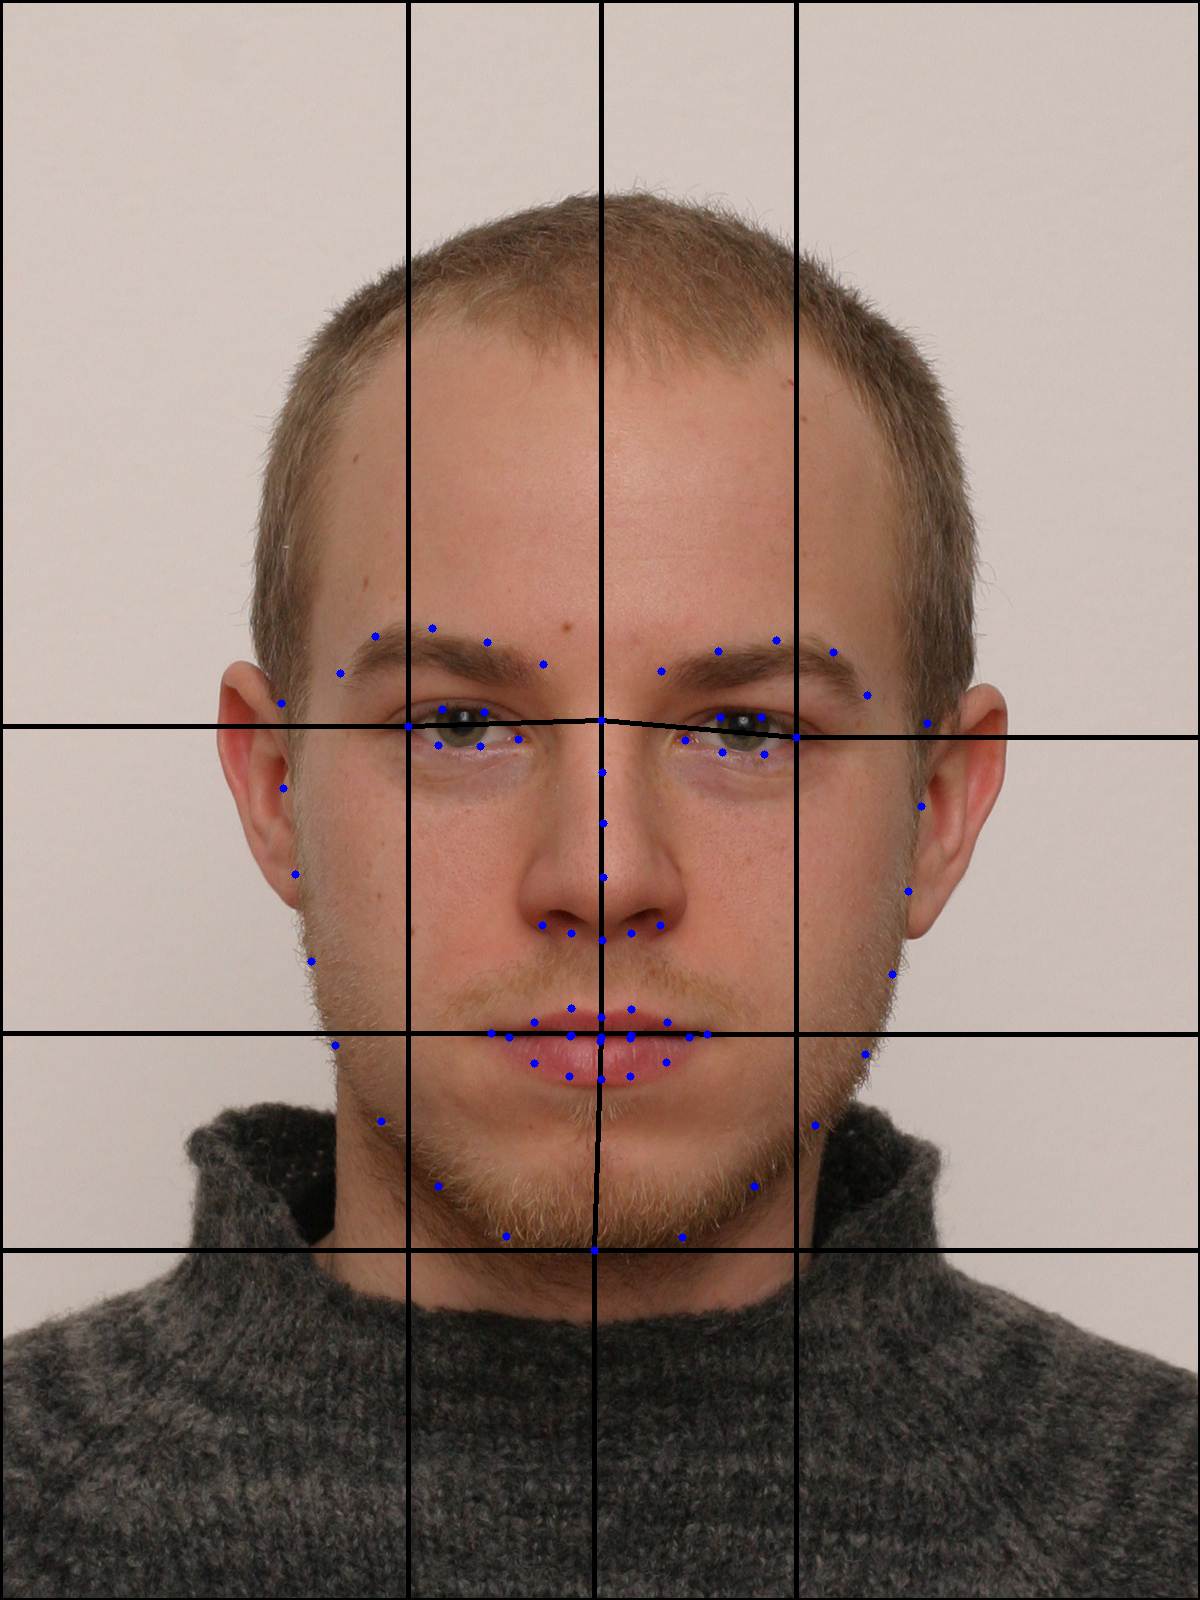
\includegraphics[width=\textwidth/2,height=\textheight/2,keepaspectratio]{001_grid}
%	\caption{Image over the landmarks (blue points) and facial grid (black lines) \label{fig:grid_img}}
%\end{figure}
%
%\section{Classification}
%
% Generally, support vector machine (SVM) tend to perform better with continuous and multidimensional features and with a large amount of samples. The features used in this case fulfill the continuity and multi dimension. Chih-Wei et. al. \cite{svm_guide} also describes a good way to optimize the use of SVM and recommend to use radial basis function (RBF) as kernel. This is why a SVM with RBF kernel is chosen for the mark classifier.  
%
%The goal with a SVM is to separate different classes by finding the best hyperplane which divides them. The hyperplane is moved such that a loss-function is minimized. RBF kernel nonlinearly maps samples into a higher dimensional space which allows the classifier to handle non-linearly separable classes. This kernel also has fewer numerical difficulties. The parameters needed for a RBF kernel i $C$ which determines the penalty parameter for the error and $\gamma$ which defines how far the influence of a single training sample reaches. \cite{svm_guide}
%
%The training data consists of the labelled facial marks provided by the supervisors at NFC. To get a good classifier, a set of discriminative features are required.
%
%\subsection{Features}
%
%The most common color space in use is the RGB system, one channel each for the red, green and blue colors. Arfika Nurhudatiana et al. \cite{torso_RPPVSM} used, among others, the minimum, maximum, and average from the RGB-channels as discriminative features. 
%
%The features extracted from the facial marks are the mean and the standard deviation from the three RGB channels and the 11 colours from the work of Joost van de Weijer et al. This results in 28 features which is used to train the classifier. 
%
%To not let some feature with greater numeric rang dominate over features with smaller range, the features need to be scaled \cite{svm_guide}. This is very important which is why the features are linearly scaled to a range from $0$ to $1$. The same scaling factor has to be used when the test data is scaled. 






  